%Version 2.1 April 2023
% See section 11 of the User Manual for version history
%
%%%%%%%%%%%%%%%%%%%%%%%%%%%%%%%%%%%%%%%%%%%%%%%%%%%%%%%%%%%%%%%%%%%%%%
%%                                                                 %%
%% Please do not use \input{...} to include other tex files.       %%
%% Submit your LaTeX manuscript as one .tex document.              %%
%%                                                                 %%
%% All additional figures and files should be attached             %%
%% separately and not embedded in the \TeX\ document itself.       %%
%%                                                                 %%
%%%%%%%%%%%%%%%%%%%%%%%%%%%%%%%%%%%%%%%%%%%%%%%%%%%%%%%%%%%%%%%%%%%%%

%%\documentclass[referee,sn-basic]{sn-jnl}% referee option is meant for double line spacing

%%=======================================================%%
%% to print line numbers in the margin use lineno option %%
%%=======================================================%%

%%\documentclass[lineno,sn-basic]{sn-jnl}% Basic Springer Nature Reference Style/Chemistry Reference Style

%%======================================================%%
%% to compile with pdflatex/xelatex use pdflatex option %%
%%======================================================%%

%%\documentclass[pdflatex,sn-basic]{sn-jnl}% Basic Springer Nature Reference Style/Chemistry Reference Style


%%Note: the following reference styles support Namedate and Numbered referencing. By default the style follows the most common style. To switch between the options you can add or remove in the optional parenthesis. 
%%The option is available for: sn-basic.bst, sn-vancouver.bst, sn-chicago.bst, sn-mathphys.bst. %  
 
\documentclass[bst/sn-nature]{sn-jnl}% Style for submissions to Nature Portfolio journals
%%\documentclass[sn-basic]{sn-jnl}% Basic Springer Nature Reference Style/Chemistry Reference Style
%\documentclass[bst/sn-mathphys,Numbered]{sn-jnl}% Math and Physical Sciences Reference Style
%%\documentclass[sn-aps]{sn-jnl}% American Physical Society (APS) Reference Style
%%\documentclass[sn-vancouver,Numbered]{sn-jnl}% Vancouver Reference Style
%%\documentclass[sn-apa]{sn-jnl}% APA Reference Style 
%%\documentclass[sn-chicago]{sn-jnl}% Chicago-based Humanities Reference Style
%%\documentclass[default]{sn-jnl}% Default
%%\documentclass[default,iicol]{sn-jnl}% Default with double column layout

%%%% Standard Packages
%%<additional latex packages if required can be included here>
\usepackage{tabularx} % Required for better table formattin
\usepackage{graphicx}%
\usepackage{multirow}%
\usepackage{amsmath,amssymb,amsfonts}%
\usepackage{amsthm}%
\usepackage{mathrsfs}%
\usepackage[title]{appendix}%
\usepackage{xcolor}%
\usepackage{textcomp}%
\usepackage{manyfoot}%
\usepackage{booktabs}%
\usepackage{algorithm}%
\usepackage{algorithmicx}%
\usepackage{algpseudocode}%
\usepackage{listings}%
%%%%

%\jyear{2021}%

%% as per the requirement new theorem styles can be included as shown below
\theoremstyle{thmstyleone}%
\newtheorem{theorem}{Theorem}%  meant for continuous numbers
%%\newtheorem{theorem}{Theorem}[section]% meant for sectionwise numbers
%% optional argument [theorem] produces theorem numbering sequence instead of independent numbers for Proposition
\newtheorem{proposition}[theorem]{Proposition}% 
%%\newtheorem{proposition}{Proposition}% to get separate numbers for theorem and proposition etc.

\theoremstyle{thmstyletwo}%
\newtheorem{example}{Example}%
\newtheorem{remark}{Remark}%

\theoremstyle{thmstylethree}%
\newtheorem{definition}{Definition}%

\raggedbottom
%%\unnumbered% uncomment this for unnumbered level heads

\begin{document}

\title[Article Title]{Exploring ChatGPT's Potential for Identifying Childbirth-Related Post-Traumatic Stress Disorder}

%%=============================================================%%
%% Prefix	-> \pfx{Dr}
%% GivenName	-> \fnm{Joergen W.}
%% Particle	-> \spfx{van der} -> surname prefix
%% FamilyName	-> \sur{Ploeg}
%% Suffix	-> \sfx{IV}
%% NatureName	-> \tanm{Poet Laureate} -> Title after name
%% Degrees	-> \dgr{MSc, PhD}
%% \author*[1,2]{\pfx{Dr} \fnm{Joergen W.} \spfx{van der} \sur{Ploeg} \sfx{IV} \tanm{Poet Laureate} 
%%                 \dgr{MSc, PhD}}\email{iauthor@gmail.com}
%%=============================================================%%

\author*[1]{\fnm{Alon} \sur{Bartal}}\email{alon.bartal@biu.ac.il}

\author[2,3]{\fnm{Kathleen M.} \sur{Jagodnik}}\email{kathleen.jagodnik@biu.ac.il}

\author[2,3]{\fnm{Sharon} \sur{Dekel}}\email{sdekel@mgh.harvard.edu}

\affil*[1]{\orgdiv{The School of Business Administration}, \orgname{Bar-Ilan University}, \orgaddress{\street{Max and Anna Web}, \city{Ramat Gan}, \postcode{5290002}, \country{Israel}}}

\affil[2]{\orgdiv{Department of Psychiatry}, \orgname{Massachusetts General Hospital}, \orgaddress{\street{Street}, \city{Boston}, \postcode{10587}, \state{Massachusetts}, \country{USA}}}

\affil[3]{\orgdiv{Department of Psychiatry}, \orgname{Harvard Medical School}, \orgaddress{\street{Street}, \city{Boston}, \postcode{10587}, \state{Massachusetts}, \country{USA}}}

%%==================================%%
%% sample for unstructured abstract %%
%%==================================%%

\abstract{Maternal mental health is a critical concern during and after childbirth, affecting both mothers and their children. 
Untreated postpartum psychopathology can result in child neglect, leading to substantial pediatric health expenses and societal costs. 
Following childbirth, some women experience childbirth-related post-traumatic stress disorder (CB-PTSD). 
While postpartum depression is routinely screened, there is no standardized protocol for identifying those at risk of CB-PTSD. 
Recent computational advances in free text analysis show promise for diagnosing psychiatric conditions.
This study explores the potential of Chat Generative Pre-trained Transformer (ChatGPT), a large language model (LLM) developed by OpenAI, for the clinical task of screening for CB-PTSD by analyzing maternal narratives of childbirth experiences.
We utilize the power of ChatGPT's \texttt{gpt-3.5-turbo-16k} LLM to classify narratives using zero-shot and few-shot learning.
Additionally, we extract the numerical vector representation (embeddings) of narratives using the \texttt{text-embedding-ada-002} model via OpenAI’s API.
Using these embeddings, we trained a densely connected feedforward neural network (DFNN) to detect CB-PTSD via narrative classification.
Our DFNN model, trained using OpenAI's embeddings, outperformed ChatGPT's zero- and few-shot learning, and six previously published models trained on mental health and clinical domains.
Understanding the connection between narrative language and post-traumatic outcomes enhances support for at-risk mothers, benefiting both mother and child.}

\keywords{ChatGPT,
Childbirth-related post-traumatic stress disorder (CB-PTSD),
Large language model (LLM),
Maternal mental health,
Narrative language,
Postpartum psychopathology
}

%%\pacs[JEL Classification]{D8, H51}

%%\pacs[MSC Classification]{35A01, 65L10, 65L12, 65L20, 65L70}

\maketitle

%====================================================================
\section{Introduction}
\label{sec: intro}
%====================================================================

Each year, approximately 140 million women give birth worldwide \cite{sommerlad2021trait}. 
For approximately one-third of this population, childbirth may be a source of significant stress or trauma, and a significant minority will develop childbirth-related post-traumatic stress disorder (CB-PTSD) \cite{dekel2020beyond}.
Historically, PTSD has been associated with military combat or severe sexual assault \cite{dekel2016trauma}. 
In recent years, however, childbirth has become increasingly acknowledged as a significant PTSD trigger \cite{dekel2020beyond,yildiz2017prevalence}.

Of the global childbearing population, approximately 6\% will manifest full CB-PTSD \cite{yildiz2017prevalence}, which translates to ~8+ million affected individuals per year. Untreated CB-PTSD is associated with negative effects in the mother and, by extension, her child \cite{van2022childbirth,dekel2019childbirth}, and these consequences carry significant societal costs \cite{lyons2022developmental,luca2019societal}. Early treatment for CB-PTSD facilitates improved outcomes.
This underscores the imperative need for effective strategies that can predict the development of CB-PTSD soon after a traumatic birth.
Currently, the evaluation of CB-PTSD relies on patients' self-reporting of symptoms.
The self-report questionnaires used in such assessments have several drawbacks that include under-reporting due to stigma, fears of infant separation, and lack of awareness that can lead to significant under-diagnoses \cite{anokye2018prevalence, jones2022postpartum}.
Therefore, relying solely on self-reported symptoms can compromise the identification of CB-PTSD.

In this context, the narrative style and language that individuals use when recounting traumatic events have been suggested to provide deep insights into their mental well-being \cite{vanaken2021keep,boyd2017multifaceted,alvarez2001linguistic}.
Research has shown that the way in which individuals remember and describe traumatic events, encompassing the language used in the narrative, is connected to the expression of their post-traumatic stress symptoms \cite{crespo2016memory}.
The words in individuals' traumatic narratives may reflect post-trauma adjustment even before deep psychological analysis occurs \cite{o2006trauma}.

Recent advancements in the field of natural language processing (NLP) computational methods show that algorithms can analyze human language and derive understanding similar to human cognition \cite{brown2020language}.
Large language models (LLMs) refer to massive Transformer models trained on extensive datasets \cite{brants2007large}.
These NLP models have achieved remarkable results in understanding contextual nuances of language in written texts \cite{brown2020language}.
NLP methods can extract and convert unstructured textual data into structured data, usable for creating machine learning (ML) classification models.
In certain circumstances, pre-trained LLMs can be used effectively without additional training or fine-tuning, a process known as zero-shot and few-shot learning \cite{brown2020language}.
In zero-shot learning, a model uses its existing knowledge to understand tasks on which it was not explicitly trained \cite{brown2020language}.
In few-shot learning, a model can make accurate predictions after being trained on a very limited dataset for a particular task  \cite{brown2020language}.

Combined with ML models, language models have been reported as useful in the classification of psychiatric conditions.
For example, the MentalBERT and MentalRoBERTa LLMs were trained to benefit the mental healthcare research community in identifying stress, anxiety, and depression mental disorders \cite{ji2021mentalbert}.
The mental-xlnet-base-cased \cite{ji2023domain} LLM was developed to identify various  mental health conditions including depression, stress, and suicidal attempts.
In both studies, the authors found that language representations pretrained in the target domain improve model performance on mental health detection tasks.
In the research field of CB-PTSD, we previously used the embeddings of sentence-transformers to train an ML classifier for identifying at-risk women \cite{bartal2023identifying}.
This model achieved an F1-score of 0.76, sensitivity of 0.8, and specificity of 0.7.
In that project, we transformed narratives to vectors and calculated the distance between each two vector-pairs affiliated with the groups of CB-PTSD vs. not-CB-PTSD, as well as between vectors affiliated with mixed groups.
More research is required to characterize how word usage in birth narratives indicates maternal mental health.

Recently, the medical community became intrigued by the capabilities of the Chat Generative Pre-trained Transformer (ChatGPT) LLM after it showcased its proficiency in passing medical board exams \cite{gordijn2023chatgpt}.
ChatGPT functions as a conversational agent proficient in following complex instructions and generating high-quality responses in diverse scenarios.
In addition to its conversational abilities, ChatGPT has demonstrated remarkable performance on various other NLP tasks, including question-answering \cite{bang2023multitask}, even in zero- or few-shot learning scenarios \cite{brown2020language}.
In these scenarios, ChatGPT was applied to new tasks with no fine-tuning using no training data (zero-shot) or a small quantity of data (few-shot) \cite{brown2020language}.

In the mental health domain, ChatGPT was able to identify a single patient with schizophrenia and recommend a treatment that aligns with current clinical standards of care \cite{galido2023case}. 
ChatGPT (GPT-3.5 and GPT-4) have shown significant language processing capabilities in the realm of mental health analysis.
For example, the performance of ChatGPT was evaluated in detecting stress, depression, and suicide, showcasing its strong capability of usefully assessing mental health texts \cite{lamichhane2023evaluation}. 
Using zero-shot analysis, the performance of ChatGPT in identifying suicide and depression suggested a promising future for LLMs for mental health \cite{amin2023will, qin2023chatgpt}.

Contrary to previous findings that ChatGPT has presented promising results in the health care domain, a recent review \cite{li2023chatgpt} reports that the current release of ChatGPT has achieved only moderate performance on a variety of clinical tests, and is unreliable for clinical deployment since it was not designed for clinical applications.
Models such as clinicalBERT \cite{alsentzer2019publicly} and BioGPT \cite{luo2022biogpt} that were trained on domain-specific content outperformed ChatGPT in clinical tasks \cite{li2023chatgpt}.

These seemingly contradictory findings highlight the current lack of understanding regarding whether ChatGPT can effectively be used for clinical assessments such as identifying women with a high risk of CB-PTSD.
To date, only a few studies (e.g., \cite{bartal2023identifying}) have explored the potential of using childbirth narratives analyzed via advanced text-based computational methods and ML for early detection of individuals showing signs of traumatic stress post-childbirth.
Therefore, understanding and analyzing traumatic narratives remains an area ripe for exploration.

This paper explores the capabilities of ChatGPT, examining its efficacy in analyzing childbirth narratives to identify potential markers of CB-PTSD. 
Through the lens of ChatGPT and associated models, we aim to bridge the gap between traumatic narratives and early detection, offering a novel approach to identifying those at risk for CB-PTSD.
To achieve this aim, we collected textual narratives of recent childbirth experiences of postpartum women.
Using OpenAI's LLMs, we tested whether the text of narratives, alone, could be used to identify postpartum women with probable CB-PTSD.
We evaluated the classification performances of three models:
Model \#1 involves zero-shot classification, and
Model \#2 involves few-shot learning.
For both Models \#1 and \#2, we used the \texttt{gpt-3.5-turbo-16k} architecture that supports analysis of long narratives.
ChatGPT (\texttt{gpt-3.5}) and \texttt{gpt-3.5-turbo} versions are essentially the same model, based on the \texttt{gpt-3.5} architecture developed by OpenAI.
However, the underlying architecture of \texttt{gpt-3.5-turbo} is more general and powerful for language modeling.
Additionally, we developed Model \#3, a densely connected feedforward neural network (DFNN) classifier that was trained and evaluated using vectors of narratives, extracted from the \texttt{text-embedding-ada-002} LLM, available via the OpenAI API.
Our Model \#3 outperformed Models \#1 and \#2, as well as six previously published models trained on clinical and mental-health domains.



%============


%Around the globe, about 140 million individuals give birth each year \cite{sommerlad2021trait}.
%For approximately one-third of these individuals, childbirth becomes a significantly stressful and potentially traumatizing event that can result in a mental illness of posttraumatic stress disorder (PTSD)\cite{dekel2020beyond}.
%Traditionally, we associate PTSD with experiences of war, combat, or severe sexual assault\cite{dekel2016trauma}.
%However, in recent years, it's increasingly acknowledged that the trauma related to childbirth can be potent enough to trigger PTSD symptoms in women post-delivery\cite{dekel2020beyond,yildiz2017prevalence}.

%Out of all individuals who give birth globally, roughly 6\% will experience full-fledged childbirth-related PTSD (CB-PTSD)\cite{yildiz2017prevalence}.
%Risk factors of CB-PTSD include complicated medical deliveries such as emergency or unscheduled cesarean delivery \cite{dekel2019delivery}, obstetric complications \cite{dekel2020beyond}, and maternal near-miss incidents\cite{england2020monitoring}.
%A noticeable racial inequality was detected in the experiences of childbirth trauma, revealing that Black and Latinx women are nearly three times more prone to experiencing an acute stress response to childbirth\cite{iyengar2022increased}.
%Overall, around 20\% of individuals in high-risk categories are likely to suffer from CB-PTSD\cite{yildiz2017prevalence}.

%The onset of CB-PTSD usually coincides with the arrival of the baby, turning the child into a potential traumatic reminder for the mother. 
%A central issue that arises from this is a disruption in the bonding process between mother and child. Problems in maternal attachment can appear during the first postpartum year and may lead to a decrease in exclusive breastfeeding \cite{kjerulff2021prospective}, thereby impacting an essential period for child development\cite{chan2020risk}. 
%Thus, CB-PTSD may obstruct early child development and contribute to significant public health expenditure.

%Recognizing individuals who are likely to develop CB-PTSD soon after a traumatic delivery is crucial for their psychological adjustment. 
%Precise screening can be the initial step in enhancing opportunities for effective interventions and resource allocation to those at risk\cite{berman2021association}.
%However, underreporting of symptoms, owing to shame, stigma, fears of infant separation, and poor awareness, poses a challenge to postpartum mental health screening\cite{anokye2018prevalence, jones2022postpartum}. 
%Hence, the evaluation of CB-PTSD that relies on patients' self-reporting of symptoms might be compromised due to the lack of introspective abilities and potential bias in reporting.

%It has been suggested that the natural language derived from spontaneous word usage can serve as an indicator of mental health and psychopathology\cite{boyd2017multifaceted}.
%The personal memory of a traumatic event plays a key role in PTSD's onset and perpetuation\cite{engelhard2019retrieving}.
%Research has shown that the way individuals remember and describe traumatic events, encompassing the language used in the narrative, is connected to the expression of their posttraumatic stress symptoms\cite{crespo2016memory}.
%Consequently, the words used in individuals' narration of the traumatic event might mirror the adjustment post-trauma, even before extensive psychological processing and interpretation take place\cite{o2006trauma}.

%Recent advancements in natural language processing (NLP) computational methods show that algorithms can analyze human language and derive understanding similar to human cognition\cite{brown2020language}.
%Combined with machine learning (ML) models, these have already been found to be useful in the classification of psychiatric conditions\cite{tsui2021natural}.

%Large language models (LLMs) refer to massive Transformer models trained on extensive datasets\cite{brants2007large}.
%These NLP models have achieved remarkable results in understanding contextual nuances of language in written texts\cite{brown2020language}.
%NLP can extract and convert unstructured textual data into structured data, usable for creating ML classification models.

%In certain circumstances, pre-trained Large Language Models (LLMs) can be used effectively without additional training or fine-tuning, process known as zero-, and few-shot learning\cite{brown2020language}.
%In zero-shot learning a model uses its existing knowledge to understand tasks it was not explicitly trained on\cite{brown2020language}.
%In other circumstances, a model can make accurate predictions after being trained on a very limited amount of data for a particular task (few-shot learning)\cite{brown2020language}.

%Generative Pre-trained Transformers (GPT) belong to a class of LLMs capable of producing human-like responses based on textual input. 
%OpenAI introduced ChatGPT (or GPT-3.5) in November 2022. 
%ChatGPT functions as a conversational agent proficient in following complex instructions and generating high-quality responses in diverse scenarios.
%In addition to its conversational abilities, ChatGPT has demonstrated remarkable performance in various other NLP tasks, including Question-answering \cite{bang2023multitask}, even in zero- or few-shot learning scenarios\cite{brown2020language}.
%In these scenarios, ChatGPT was applied to new tasks with no fine-tuning using a small amount of data.

%In an example that is highly relevant to this study, we identified CB-PTSD by analyzing narratives \cite{bartal2023identifying}. 
%They used Sentence-Transformer Language Model (LLMs) in combination with a machine learning (ML) classifier, achieving an F1-score of 0.76, a sensitivity of 0.8, and a specificity of 0.7.
%The authors transformed narratives to vectors and calculated the distance between each two vector-pairs affiliated with the CB-PTSD, or not groups; as well as between vectors affiliated with mixed groups.
%However, much work is needed for understanding whether word usage in birth narratives can be an indicator of maternal mental health. 
%Additionally, there is a lack of understanding regarding whether LLMs (such as ChatGPT) can effectively identify individuals with a high risk of CB-PTSD.
%To date, only a few studies, including our work \cite{bartal2023identifying}, have explored the potential of using childbirth narratives along with advanced text-based computational methods and machine learning (ML) for early detection of individuals showing signs of traumatic stress post-childbirth.
%Therefore, this area requires substantial further investigation.

%We collected textual narratives of recent childbirth experiences of postpartum individuals.
%Using the OpenAI's LLMs, we tested whether the text of narratives, alone, could be used to identify postpartum individuals with probable CB-PTSD.
%We evaluated the classification performances of three models.
%Model \#1 involves zero-shot classification,
%Model \#2 involves few-shot learning.
%For both Models \#1 and \#2, we used the \texttt{gpt-3.5-turbo-16k} architecture.
%ChatGPT and \texttt{gpt-3.5-turbo} are essentially the same model, based on the \texttt{gpt-3.5} architecture developed by OpenAI.
%However, the underlying architecture of \texttt{gpt-3.5-turbo} is more general and powerful for language modeling.
%Additionally, we developed Model \#3, a ML classifier that was trained and evaluated using vectors of narratives extracted from the \texttt{text-embedding-ada-002} LLM, available via the OpenAI API.


%====================================================================
\section{Materials and Methods}
%====================================================================
\subsection{Study Design}
%====================================================================
This research was part of two broader studies.
The first study examined the impact of the COVID-19 pandemic on the childbirth experience and subsequent maternal mental health.
The second study examined CBEx...

We gathered data from individuals aged 18 and over who had given birth to a live baby within the past six months.
These individuals shared details about their mental health and childbirth experiences through an anonymous online questionnaire.
They were given the opportunity to recount their childbirth stories at the end of the survey. 
These narratives were collected, on average, 2.50±1.78 months post-childbirth (ranging from 0.02 to 8.34 months). 
We recruited participants from April 2, 2020, through December 29, 2020, via hospital bulletins, social media platforms, and professional associations.
Both projects were granted an exemption by the Human Research Committee of Partners Healthcare (Massachusetts General Brigham).

Our participant group consisted of ??? individuals who shared their childbirth narratives. 
Of these, 1,406 completed a PTSD symptom questionnaire, with 1,295 providing detailed childbirth narratives of 30 words or more to allow meaningful learning of word patterns. 
The participants had an average age of 32.00 4.43 years and a gestational age of 38.98 1.71 weeks. 
It's worth noting that 53.1\% were first-time mothers, and 69.6\% had vaginal births. 
Additionally, 10\% (or 190 participants) screened positive for PTSD, according to the PTSD Checklist for The Diagnostic and Statistical Manual of Mental Disorders, Fifth Edition, PCL-5 $=31$. 
Table \ref{tbl:...} outlines the demographics and childbirth details for participants with and without a positive PTSD screen, all of which were self-reported by the subjects.

\subsection{Measures}
We gathered narratives of childbirth in the form of open-ended, unstructured written accounts, highlighting each participant's personal and recent experience of childbirth. These narratives were procured using a free recall methodology, where participants were asked to provide a concise account of their recent childbirth experience, focusing specifically on the most distressing elements, if any. This focus on the most distressing parts aligns with standard procedures used in non-postpartum trauma sequelae research.

We assessed PTSD symptoms associated with childbirth using the PCL-5 tool, a common self-report measure used to ascertain the presence and severity of the 20 DSM-5 PTSD symptoms after a designated traumatic event over the preceding month. 
Participants were guided to report symptoms linked to their recent childbirth experience. The PCL-5 is widely recognized for its strong alignment with diagnostic assessments by clinicians and is used to establish a provisional PTSD diagnosis (i.e., a presumptive disease state without a formal diagnosis).
The clinical cutoff for this measure is reported to be 31.
The reliability of this tool was high, as indicated by a Cronbach $\alpha =0.91$.

%==========================================================
\subsection{Narrative Analysis}
%==========================================================
We compared the following three developed models by utilizing the \texttt{gpt-3.5-turbo-16k} LLM with OpenAI's API. Fig. \ref{fig:models} present a summary of the three models evaluated in this study.
The \texttt{gpt-3.5-turbo} LLM developed by OpenAI, is a powerful transformer model that excels in natural language understanding and generation tasks.
It's variation of \texttt{gpt-3.5-turbo-16k} has the same capabilities as the standard \texttt{gpt-3.5-turbo} model but can process four times longer narratives of up to 16384 tokens.

\textbf{Model \#1 -- zero-shot classification} with no previous examples given to the model. 
We designed a prompt that includes a description of the task, followed by the narrative to be classified.
The category associated with the response that the model is most confident in was `1' (CB-PTSD) or `0' (No CB-PTSD) as the predicted class for the narrative.
We experimented with several versions of prompts.
For brevity sake, only the prompt that yielded the best results is presented (Table \ref{tbl:prompts}).
Using OpenAI's API, we sent this prompt to the \texttt{gpt-3.5-turbo-16k} model with `temperature'$=0$ variable, which returned a response to each prompt.
A temperature of 0 will make the model deterministic, i.e., always choosing the most likely next token in the sequence.


\begin{table}
\centering
\caption{Prompts for zero- and few-shot learning using ChatGPT.}
\label{tbl:prompts}
\begin{tabularx}{\textwidth}{lX}
\hline
Model     & Prompt   \\ 
\hline
Zero-Shot & 
``You are a Psychiatrist specialized in diagnosing and treating Post Traumatic Stress Disorder (PTSD). I will provide you with a narrative written by a woman describing her birth experience. Your task is to decide whether this woman is of high risk of PTSD (Label 1), or lower risk of PTSD (Label 0). Do not write anything but '1' or '0'.
\#\#\# 
\textless{}Text\textgreater{}: ''\{text\}''
\\
\hline
Few-Shot  & 
``You are a Psychiatrist specialized in diagnosing and treating Post Traumatic Stress Disorder (PTSD). I will provide you with a narrative written by a woman describing her birth experience. Your task is to decide whether this woman is of high risk of PTSD (Label 1), or lower risk of PTSD (Label 0). Do not write anything but '1' or '0'. Here are a few examples of text with their associated class labels as '1' (PTSD), or '0' (No-PTSD). 
\textless{}Text\textgreater{}: ''\{sick\_narrative\}'' 
\textless{}Label\textgreater{}: 1
\#\#\# 
\textless{}Text\textgreater{}: ''\{healthy\_narrative\}''
\textless{}Label\textgreater{}: 0 
\#\#\#
\textless{}Text\textgreater{}: ''\{text\}''
\\
\hline
\end{tabularx}
\end{table}


\textbf{Model \#2 -- few-shot classification.}
We provided two narratives and their associated labels in a conversation format to guide the model towards the classification task (Table \ref{tbl:prompts}). 
The \texttt{gpt-3.5-turbo-16k} model with `temperature'$=0$, then used these examples to classify the expected output for the subsequent narrative. 
Increasing the number of examples up to four, provided similar model performances.

\textbf{Model \#3 -- training a ML classifier.} 
We trained a ML model using the embeddings of OpenAI's model (\texttt{text-embedding-ada-002}) to classify narrative as markers of endorsement, or no-endorsement of CB-PTSD. 
Appendix \ref{secA1} presents the four steps to build and test Model \#3, summarized in Fig. \ref{fig:dfnn}.

In Step \#1 of Appendix \ref{secA1}, we label narratives associated with PCL-5 $\geq 31$ as `CB-PTSD' (Class 1; 190 individuals), else `no CB-PTSD' (Class 0; 1105).

In Step \#2, we discarded narratives with $< 30$ words and balanced the dataset using down-sampling by randomly sampling the majority Class 0 to fit the size of the minority Class 1, resulting in 190 narratives in each class.
We constructed the Train and Test datasets as described in Step \#2, resulting in 170 narrative is each class.

To identify similar or contextually relevant narratives, in Step \#3 we adopted the approach, used in \cite{bartal2023identifying}.
This approach analyzes pairs of narratives as training examples, thus substantially increasing the number of training examples.
We created three sets of sentence-pairs using the train set:
Set \#1: All possible pairs of sentences $(C(n,r) = C(1720,2) = 14365)$ in Class 1 (CB-PTSD).
Set \#2: All possible pairs of sentences (14365) in Class 0.
Set \#3: Pairs of sentences (28730), one randomly selected from Class 1 and another randomly selected from Class 0.
We labeled sets \#1 and \#2 as positive examples as they contained semantically or contextually similar pairs of sentences (i.e., either a pair of narratives of individuals with, or without CB-PTSD).
We labeled set \#3 as negative examples as it contained pairs of non-semantically or non-contextually similar pairs of sentences. 
This data augmentation process produced 57460 training examples in the Train set.

Next, we mapped each narrative using the \texttt{text-embedding-ada-002} model into a 1536-dimensional vector.
Lastly, we computed the Hadamard product ($\circ$) \cite{davis1962norm} among each of the 57460 embedding (emb) vectors of pair of sentences $(u,v)$ in sets \#1 to \#3 of the Train set (Step 3.1), such that $z=(emb(u) \circ emb(b))$ (Appendix \ref{secA1}, Step 2).

Finally, using the 57460 vectors, following the modeling approach in \cite{bartal2023identifying}, we trained a deep feedforward neural network (DFNN) model to classify pairs of sentences in sets \#1 to \#3 as semantically similar or not.
For training, we used the Keras Python library and constructed a DFNN with an input layer of 1536 neurons, 2 hidden layers of 400 and 50 neurons, and an output neuron.
All layers had a rectified linear unit activation function, except the output neuron with a Sigmoid activation function.
We used 50 epochs, applying the Adam optimizer with a learning rate of $1e^{-4}$, batch size of 64, and binary cross-entropy loss to monitor training performance.
To avoid overfitting, we stopped training when there was no loss improvement for 3 consecutive epochs.
We used 20\% of the Train dataset for validation during the training process.

Steps \#1 to \#3 of Model \#3 (Appendix \ref{secA1}) were repeated 10 times to capture different narratives for creating an accurate representation of classes 0 and 1.


\textbf{Model evaluation.}
In Step \#4, Models \#1 and \#2 were evaluated on the entire dataset.
Model \#3 was trained on a Train set and evaluated on a Test set.
This process was repeated 10 times similar to a 10-fold cross validation process.
We tested and compared the performances of Model \#1 to \#3, using (1) the F1 score, which is a measure integrating precision (positive predictive value) and recall (sensitivity), and (2) the area under the curve (AUC).

\begin{figure}
    \centering
    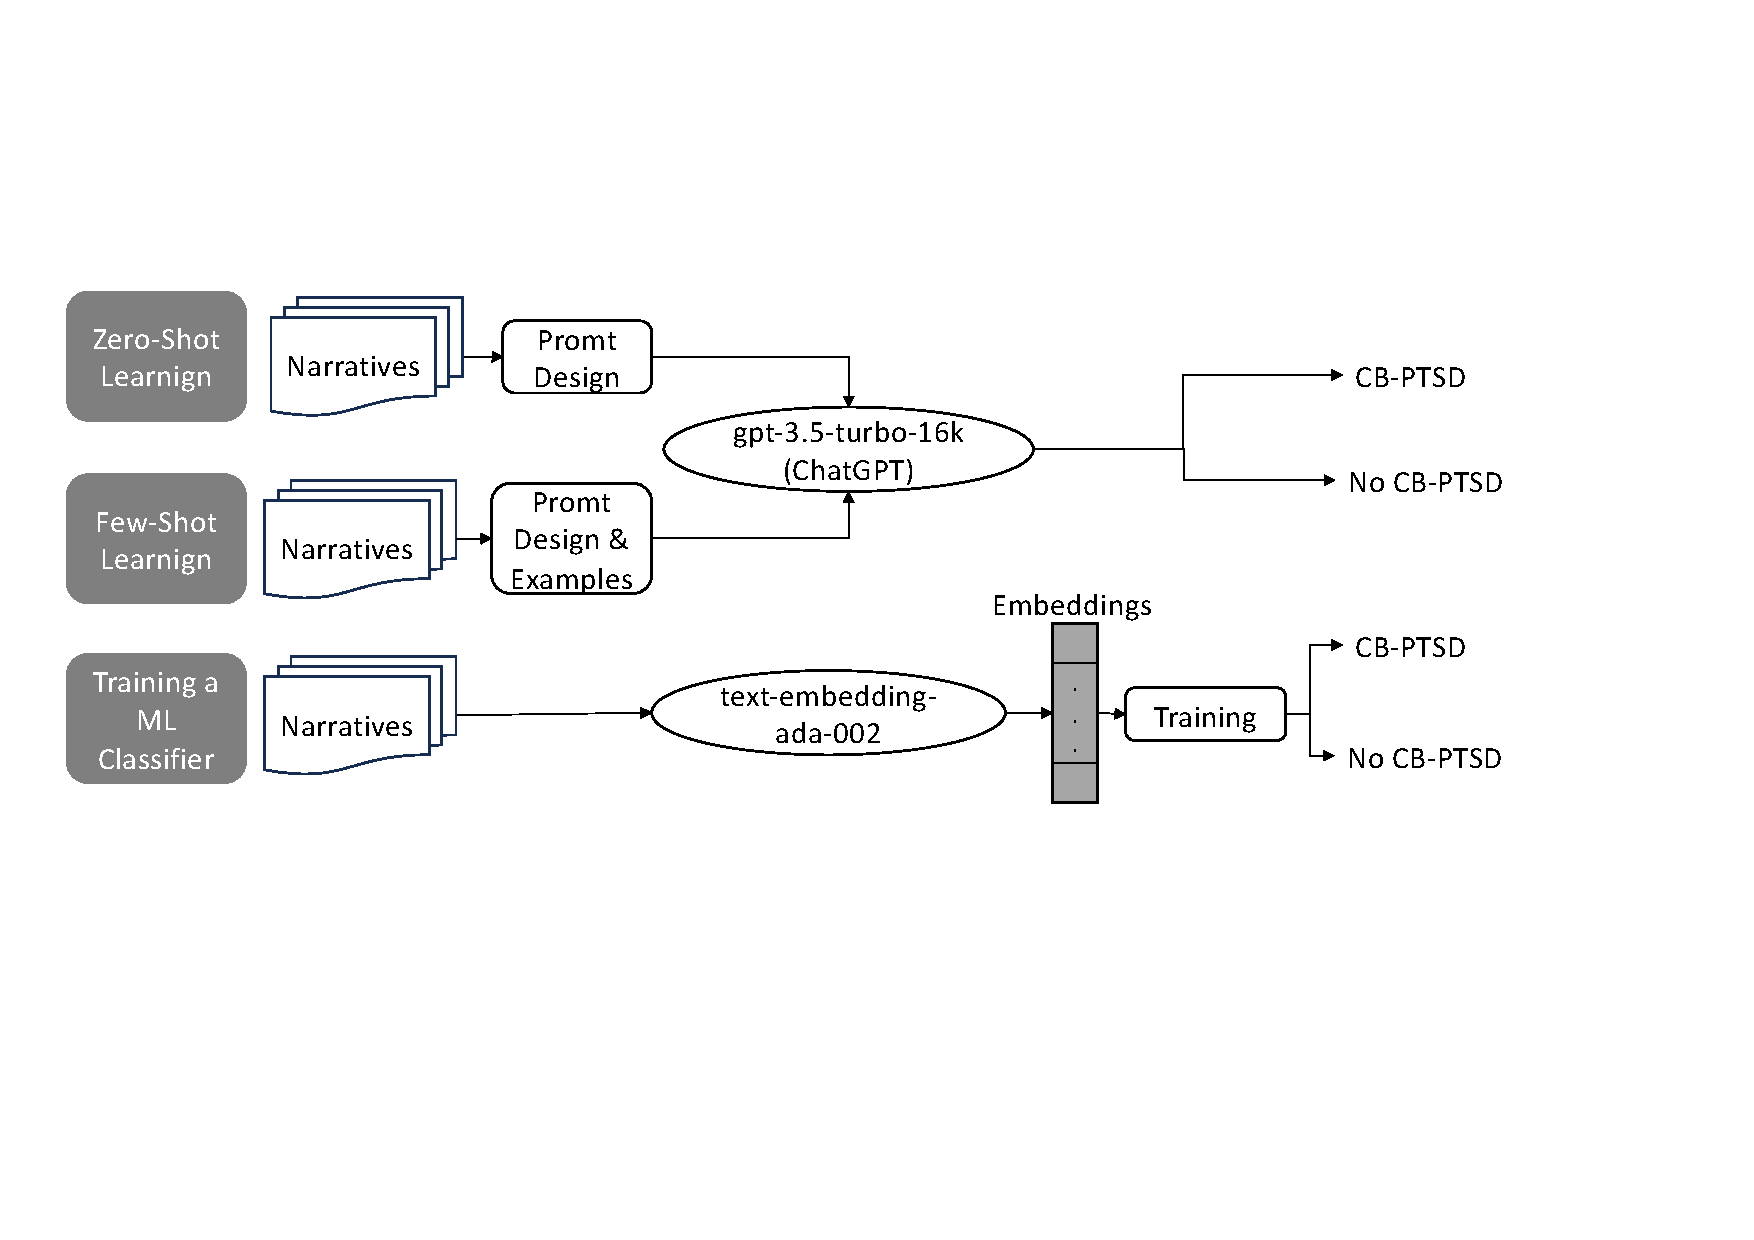
\includegraphics[scale=0.5, trim={1cm 7cm 4cm 5cm}, clip]{images/Fig_models_architecture.pdf}
    \caption{The three models employed in this study via OpenAI's API: (1) Model \#1 utilizes \texttt{gpt3.5-turbo-16k} for zero-shot classification, 
    (2) Model \#2 utilizes \texttt{gpt3.5-turbo-16k} for few-shot learning, and
    (3) Model \#3 utilizes the \texttt{text-embedding-ada-002} model to train a neural network machine learning (ML) model to screen via classification, for CB-PTSD.
    We also use Model \#3 with difference embeddings.}
    \label{fig:models}
\end{figure}

%====================================================================================
\section{Results}
%====================================================================================

Following the data processing (Steps \#1 and \#2, Appendix \ref{secA1}), for Class 1 (CB-PTSD) and Class 0 (no CB-PTSD), the mean and median word counts were 191.91 and 142, and 154.61 and 106, respectively.

The results of applying Model \#1 to \#3 to the narrative datasets are presented in Table \ref{tbl:performances}. 
Model \#3 outperformed all other models in terms of AUC, F1 score, sensitivity, and specificity.
All models rely only on textual features to identify CB-PTSD.

\begin{table*}[ht]
\centering
\caption{Comparison of models' performance classification results on the combined Dataset 1 and Dataset 2.
        Model \#1 was evaluated on the combined dataset. 
        Model \#2 was evaluated on the combined dataset except two training examples that were discarded.
        Models \#3 was evaluated on the Test set of the combined dataset.}
\label{tbl:performances}
\begin{tabular}{lllll}
\hline
Model                        & AUC   & F1-score & \begin{tabular}[c]{@{}l@{}}Sensitivity \\ (Recall)\end{tabular} & Specificity \\
\hline
Model \#1                    &  0.60  & 0.33 & 0.20   & 0.99        \\
Model \#2                    &  0.60  & 0.38 & 0.24   & 0.96        \\
Model \#3                    &  0.80  & 0.81 & 0.85   & 0.75         \\
\hline
\end{tabular}
\end{table*}


The results from ChatGPT Model \#1 and Model \#2 highlight a common issue: these models struggle to classify narratives in a specific domain of expertise because they have not been trained on it. 
In other words, they are pre-trained models that have not been tailored to the specialized subject matter.
Model \#3, however, successfully tackled this problem and outperformed the other models.
It did so by using a larger dataset of 57,460 examples and training a machine learning model for the specific classification task.
This specialized training involved using embeddings to create a classification system designed to detect CB-PTSD.
By training the model this way, it was better suited for the specialized task at hand.

As reported in Table \ref{tbl:performances} and, in particular, regarding the F1 score (0.81) and AUC (0.8), our model for CB-PTSD classification derived from birth narratives achieved overall good performance (Fig. \ref{fig:roc_auc}).


\begin{figure}
    \centering
    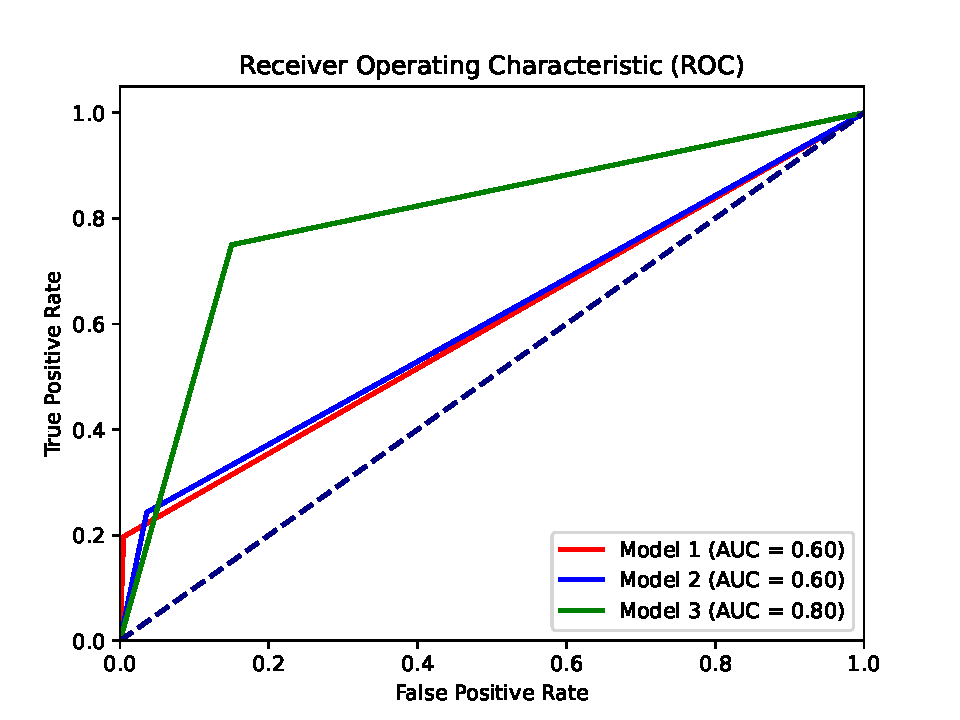
\includegraphics[scale=0.8, trim={0cm 0cm 0cm 1.35cm}, clip]{images/roc_curve.pdf}
    \caption{Comparison of Receiver Operating Characteristic (ROC) curves of binary classification models \#1 to \#3.
    The three models directly predict class labels (0 or 1) instead of probabilities. 
    The 'stepped' appearance of the ROC curves is due to the models' binary output, which allows for only 0 or 1 thresholds.
}
    \label{fig:roc_auc}
\end{figure}

It was found that ChatGPT's performance in the biomedical domain are moderate or satisfactory in various tests \cite{li2023chatgpt}.
Currently, ChatGPT is not reliable for clinical deployment due to its design, which doesn't prioritize clinical applications \cite{li2023chatgpt}.
Research indicates that specialized natural language processing models trained on bio-medical datasets remain the recommended approach for clinical uses \cite{li2023chatgpt}.

Therefore, to evaluate our model, we compared the performance of our Model \#3 with different embeddings generated by 6 LLMs that were trained on the clinical and mental-health domains (Table \ref{tbl:compar}).
We used the HuggingFace repository \cite{wolf2019huggingface} with Python coding.
The models that we compared (Table \ref{tbl:compar}) were evaluated using two Evaluation Methods on the dataset published in \cite{bartal2023identifying}.

Evaluation method 1 -- we fine-tuned each of the 6 evaluated LLMs on a downstream task of classifying narratives as CB-PTSD (Class 1), or not (Class 0).
We used 30\%-70\% of the data from training and testing respectively.
The results show F1-score lower than 0.2 for all models.

Evaluation method 2 -- 
Following Step 2 of Appendix \ref{secA1}, we split the Train and Test sets 10 times (similar to a 10-fold cross validation process).
The results show (Table \ref{tbl:compar}) that our Model \#3 with OpenAI's embeddings outperformed Model \#3 with other embeddings of LLMs (including embeddings of LLMs trained on clinical and mental-health domains) in identifying CB-PTSD using narrative data only.

\begin{table*}[]
\centering
\caption{Comparative performance analysis with different embeddings in Model \#3 (Appendix \ref{secA1}).
The average performance results of the 10-fold cross-validation process conducted on the same analyzed dataset that was used in \cite{bartal2023identifying} are presented.
OpenAI's embeddings in Model \#3, outperform all other embeddings in Model \#3, demonstrating superior ability in identifying CB-PTSD using narrative data only.
Results are ordered by a descending F1-score value.}
\label{tbl:compar}
\begin{tabular}{lllll}
\hline
Model   & AUC  & F1-score & \begin{tabular}[c]{@{}l@{}}Sensitivity\\ (Recall)\end{tabular} & Specificity \\ 
\hline                                              %AUC      F1       Sens    Spec
Model \#3                                           & 0.80  & 0.82   & 0.81  & 0.72        \\
all-mpnet-base-v2 \cite{bartal2023identifying}      &0.75   & 0.76   & 0.80  & 0.70         \\
mental-roberta-base \cite{ji2021mentalbert}         & 0.67  & 0.71   & 0.80  & 0.55        \\
mental-xlnet-base-cased \cite{ji2023domain}         & 0.65  & 0.70   & 0.80  & 0.50        \\
Bio\_ClinicalBERT \cite{alsentzer2019publicly}      & 0.65  & 0.63   & 0.60  & 0.70        \\
biogpt \cite{luo2022biogpt}                         & 0.62  & 0.59   & 0.55  & 0.70        \\
mental-bert-base-uncased \cite{ji2021mentalbert}    & 0.63  & 0.58   & 0.60  & 0.70        \\
\hline
\end{tabular}
\end{table*}


%========================================================================================
\section{Discussion}
\label{sec:discussion}
%========================================================================================
In our research, we concentrated on leveraging childbirth narratives to discern probable instances of childbirth-related posttraumatic stress disorder (CB-PTSD) using sophisticated natural language processing (NLP) and machine learning (ML) methodologies. 
Through an examination of several model variations of ChatGPT, we discerned the complexities inherent in classifying narratives pertaining to maternal mental health.
While Models \#1 (zero-shot learning) and \#2 (few-shot learning) that utilize the pre-trained ChatGPT model, exhibited limitations, Model \#3, drawing from OpenAI's GPT-3 embeddings (\texttt{text-embedding-ada-002}), showcased superior prowess in analyzing maternal mental health narratives.

Notably, Model \#3's performance surpasses both the basic implementations of ChatGPT and other LLMs rooted in clinical and mental-health domains, shedding light on its potential to offer richer insights into maternal mental health post-traumatic childbirth. However, as evidenced by Table \ref{tbl:performances}, ChatGPT, in its current iteration (\texttt{gpt-3.5-turbo-16k}), manifests average results, reinforcing its non-specialized nature for clinical applications. 
Existing evaluations, encompassing ours, frequently categorize ChatGPT as not fit-for-purpose for healthcare, with its applications mostly limited to controlled research settings.

Our Model \#3's capability, gauged across the two datasets, registers an 85\% sensitivity in pinpointing CB-PTSD cases based on narrative language and a specificity of 70\%. 
This model's reliance on childbirth narratives presents an efficient mechanism for data collection during the vulnerable postpartum stage, circumventing potential pitfalls of using only medical records.

The importance of prompt CB-PTSD screening cannot be overstated.
Despite the pressing need, standardized CB-PTSD screening protocols remain elusive in medical institutions. 
Early interventions are pivotal to preempt the progression of these disorders to chronic stages, complicating treatment.

Comparatively, while ML-driven CB-PTSD classification research remains in its infancy, Model \#3's outperforms previously established models, such as the one delineated in \cite{bartal2023identifying}.
Our unique approach, hinging on organic childbirth narratives, introduces an innovative, patient-friendly data acquisition method, fostering self-expression and therapeutic narrative creation.

Our technique introduces a resource-efficient and nonintrusive data collection mechanism, emphasizing childbirth narratives. Preliminary assessments based on these narratives can pre-emptively identify high-risk individuals, ensuring timely medical intervention.
The proposed model, besides fitting seamlessly into routine obstetric care, can serve as a foundation for commercial product development, facilitating its mainstream adoption. 
Importantly, it creates avenues to probe and address racial and ethnic disparities linked to childbirth trauma.

Although promising, our study has several constraints. 
The potential enhancement of our model with patient self-reports remains unexplored. 
Additionally, the employment of the PCL-5 measure, albeit well-validated, was applied before CB-PTSD's definitive confirmation in some instances, and clinician evaluations were overlooked. 
A broader representation beyond middle-class American women is imperative to ensure a holistic and universally applicable tool.

Looking forward, we advocate for two principal enhancements to our model:
(i) Specific fine-tuning of ChatGPT for CB-PTSD narrative language, optimizing embedding vector representation; and 
(ii) The assimilation of supplementary data forms, like electronic medical records.
Such augmentations can refine performance metrics, fortifying the role of computational methodologies in maternal mental health evaluation.


%-------------------------------------------------------------------------------------
\section{Conclusions}
\label{sec:conclusions}
%-------------------------------------------------------------------------------------
In this investigation, we provide a pioneering demonstration of the utility of textual data from childbirth narratives in the early detection of maternal PTSD post-childbirth. 
Harnessing advanced NLP and ML, we underscore the potential of these narratives in advancing maternal mental health assessments.
It is evident that an untrained ChatGPT falls short in clinical diagnosis of CB-PTSD.
The profound implications of our findings not only spotlight the pressing public health concerns surrounding psychiatric challenges during maternal transition but also beckon a deeper dive into optimizing these tools.
While our results are promising, they also signal the imperative to address the limitations and refine the methodologies. 
As we tread this path, the horizon seems ripe with possibilities for a future where technology seamlessly aids the timely identification and support for mothers facing post-childbirth mental health challenges.

\backmatter

%-------------------------------------------------------------------------------------
\bmhead{Supplementary information}
%-------------------------------------------------------------------------------------
The code associated with this study is publicly available on GitHub at https://github.com/bartala/ChatCB-PTSD.

%-------------------------------------------------------------------------------------
\bmhead{Acknowledgments}
%-------------------------------------------------------------------------------------
The authors would like to thank the DSI institute in Bar-Ilan University for partialy funding this project.

\section{Declarations}

Some journals require declarations to be submitted in a standardised format. Please check the Instructions for Authors of the journal to which you are submitting to see if you need to complete this section. If yes, your manuscript must contain the following sections under the heading `Declarations':

\begin{itemize}
\item Funding
\item Conflict of interest/Competing interests (check journal-specific guidelines for which heading to use)
\item Ethics approval 
\item Consent to participate
\item Consent for publication
\item Availability of data and materials
\item Code availability 
\item Authors' contributions
\end{itemize}

\noindent
If any of the sections are not relevant to your manuscript, please include the heading and write `Not applicable' for that section. 


\begin{appendices}
%======================================================================
\section{Steps to Build and Test Model \#3 of This Study}
\label{secA1}
%======================================================================
The following four steps describe how we built and tested Model \#3:

\textbf{Step 1. Define a PCL-5 cutoff score.} 
We labeled each narrative as Class 1: probable CB-PTSD (`CB-PTSD') based on PCL-5 $\geq 31$, or Class 0: no probable CB-PTSD (`No CB-PTSD') based on PCL-5 $<31$.

\textbf{Step 2. Data preparation.}
We discarded narratives with $< 30$ words from the dataset. 
To handle the imbalance in the analyzed data set (due to the small representation of cases with PCL-5 $\geq 31$), we randomly sampled the majority Class 0 to fit the size of the minority Class 1.
Using the balanced dataset, we randomly selected 70\% of the narratives to train our model and 30\% to test our model.
This step was repeated 10 times.

\textbf{Step 3. Develop a machine learning classifier that utilizes NLP features.}
Using the train set, we analyze pairwise narrative (sentence) that learns to identify semantically or contextually similar pairs of sentences.
First, each sentence ($S_i$) is mapped onto a fixed-size embedding vector using the \texttt{text-embedding-ada-002} model via OpenAI API that we denote $emb(S_i)$. 
Thus, $S_i$ is encoded to a vector using a function $emb(S_i)$.
To learn if two sentences are semantically or contextually similar, we train a classifier to decide if their Hadamard product (denoted: `$\circ$') \cite{davis1962norm} indicates that both vectors affiliate with the same class or not.
Given a sentence $S_a$ not present during training, a sentence $S_1 \in$ Class 1, and a sentence $S_0 \in$ Class 0, then $S_a \in$ Class 1 if the probability of Class 1 affiliation when applying our developed model to the Hadamard product ($emb(S_a)\circ emb(S_1)$) is higher than the probability of Class 0 affiliation when applying our developed model to $emb(S_a)\circ emb(S_0)$.

This approach allowed us to generate multiple training examples since there are $n(n-1)/2$ possible combinations for $n$ sentences, thus addressing the challenge of training an ML model with a low number of examples, as in Class 1.
The following three substeps describe the model development.
\begin{enumerate}
    \item 
    Each pair of sentences in Class 1, and each pair of sentences in Class 0, was labeled as positive examples, indicating semantically or contextually similar sentences of individuals with (Set \#1), or without (Set \#2) CB-PTSD, respectively. 
    Next, negative examples (Set \#3) of the same size as the positive examples sets ($||$Set \#1$|| + ||$Set \#2$||$) were created by randomly selecting pairs of sentences, one from Class 1, and the other from Class 0, indicating semantically or contextually nonsimilar sentences.
    \item 
    Using the \texttt{text-embedding-ada-002} model, each sentence was mapped into a dense vector space. 
    Then, for each Set \#1 to \#3, we computed a vector $z$ of the absolute elementwise difference between the embedding $(emb)$ of each pair of sentences $(u,v)$, selected in Substep 1, $z=(emb(u)\circ emb(v))$.
    \item 
    Train a densely connected feedforward neural network (DFNN) to classify pairs of sentences (by processing vector $z$) as semantically similar or not.
\end{enumerate}

\textbf{Step 4. Test model performance.}
We compared the performance of Model \#3 to the model in \cite{bartal2023identifying}, as well as to Model\#2 and Model \#3.
We report the area under the receiver operating characteristic curve (AUC), F1-score, Sensitivity, and Specificity measures on the Test set. 
To test Model \#3 on a newly unseen narrative $S$ in the Test set, we first compute its embeddings.
Next, we calculate the average embedding vector $(\overline{v}_n)$ of all Train narratives in Class 0, and the average embedding vector $(\overline{v} _p)$ of all Train narratives in Class 1.
To decide the class of S, we compute $z_n=(emb(S)\circ \overline{v}_n)$, and $z_p=(emb(S)\circ \overline{v}_p)$. 
Then, we apply Model \#3 (denoted as $f(x)$) to $z_n$ and $z_p$, and compare its output, i.e., compare the likelihood of similarity of $emb(S)$ to $\overline{v}_p$ with the likelihood of similarity of $emb(S)$ to $\overline{v}_n$.
If $f(z_p)> f(z_n)$, we say that $S \in$ Class 1, else $S\in$ Class 0. 
Intuitively, our model should assign a higher likelihood of similarity between an embedded narrative of an individual with CB-PTSD to the vector $\overline{v}_p$ than to the vector $\overline{v}_n$.


\begin{figure}
    \centering
    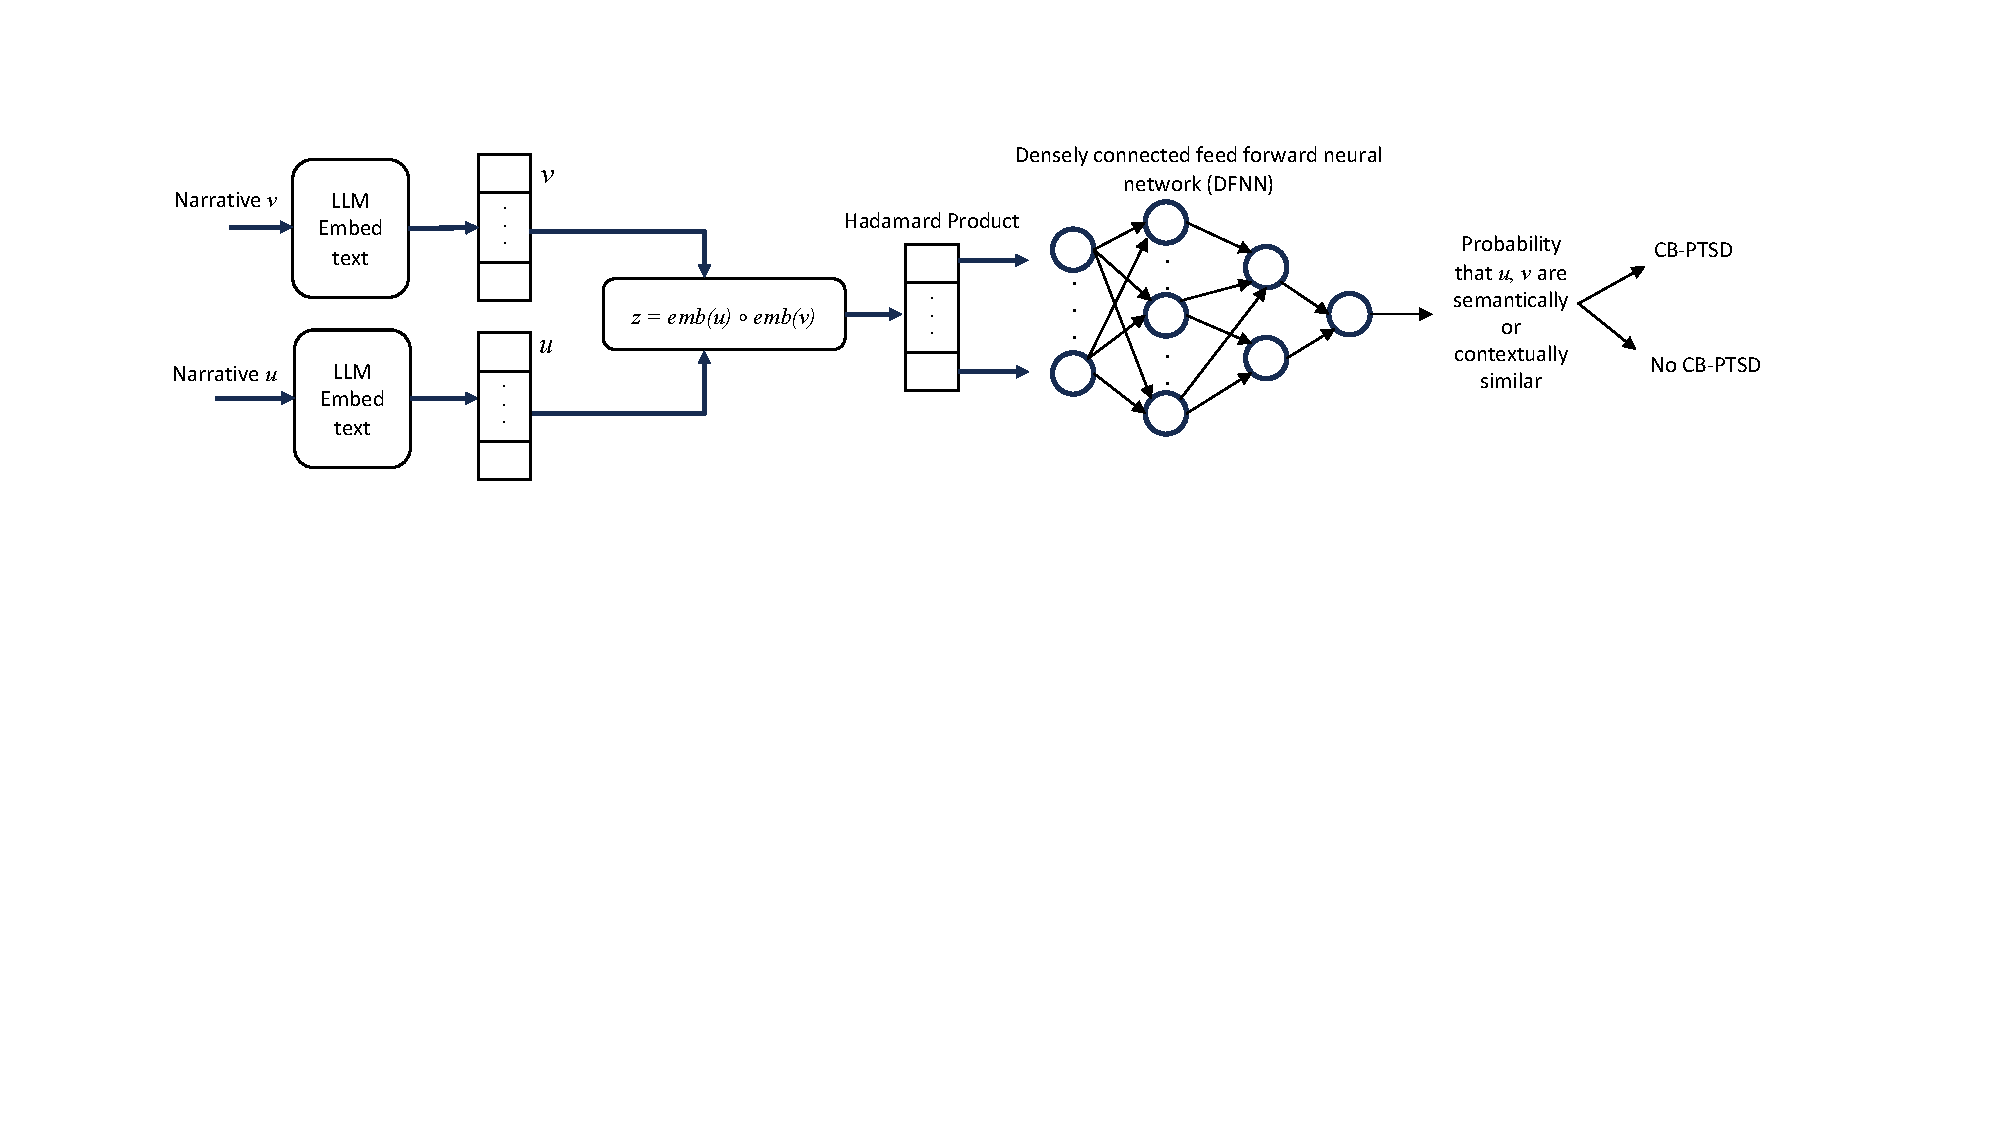
\includegraphics[scale=0.5, trim={0cm 0cm 0cm 0cm}, clip]{images/model.pdf}
    \caption{The modeling approach for classifying pairs of narratives associated with individuals with or without CB-PTSD.}
    \label{fig:dfnn}
\end{figure}


%%=============================================%%
%% For submissions to Nature Portfolio Journals %%
%% please use the heading ``Extended Data''.   %%
%%=============================================%%

%%=============================================================%%
%% Sample for another appendix section			       %%
%%=============================================================%%

%% \section{Example of another appendix section}\label{secA2}%
%% Appendices may be used for helpful, supporting or essential material that would otherwise 
%% clutter, break up or be distracting to the text. Appendices can consist of sections, figures, 
%% tables and equations etc.

\end{appendices}

%%===========================================================================================%%
%% If you are submitting to one of the Nature Portfolio journals, using the eJP submission   %%
%% system, please include the references within the manuscript file itself. You may do this  %%
%% by copying the reference list from your .bbl file, paste it into the main manuscript .tex %%
%% file, and delete the associated \verb+\bibliography+ commands.                            %%
%%===========================================================================================%%

\bibliographystyle{bst/sn-nature} 
\bibliography{sn-bibliography}% common bib file
%% if required, the content of .bbl file can be included here once bbl is generated
%%\input sn-article.bbl


\end{document}
